\documentclass[11pt]{exam}

\usepackage{amssymb, amsmath, amsthm, mathrsfs, multicol, graphicx}
\usepackage{tikz, pgfplots}


\def\d{\displaystyle}
\def\?{\reflectbox{?}}
\def\b#1{\mathbf{#1}}
\def\f#1{\mathfrak #1}
\def\c#1{\mathcal #1}
\def\s#1{\mathscr #1}
\def\r#1{\mathrm{#1}}
\def\N{\mathbb N}
\def\Z{\mathbb Z}
\def\Q{\mathbb Q}
\def\R{\mathbb R}
\def\C{\mathbb C}
\def\F{\mathbb F}
\def\A{\mathbb A}
\def\X{\mathbb X}
\def\E{\mathbb E}
\def\O{\mathbb O}
\def\pow{\mathscr P}
\def\inv{^{-1}}
\def\nrml{\triangleleft}
\def\st{:}
\def\~{\widetilde}
\def\rem{\mathcal R}
\def\iff{\leftrightarrow}
\def\Iff{\Leftrightarrow}
\def\and{\wedge}
\def\And{\bigwedge}
\def\AAnd{\d\bigwedge\mkern-18 mu\bigwedge}
\def\Vee{\bigvee}
\def\VVee{\d\Vee\mkern-18 mu\Vee}
\def\imp{\rightarrow}
\def\Imp{\Rightarrow}
\def\Fi{\Leftarrow}


\def\bar{\overline}

%\pointname{pts}
\pointsinmargin
\marginpointname{pts}
\marginbonuspointname{ bns pts}

\addpoints
\pagestyle{headandfoot}
%\printanswers


\header{MATH 131}{\bf\large Learning Target 6 Quiz}{Fall 2025}
\runningfooter{}{}{Version \version}
\extrafootheight{-.45 in}



\begin{document}
\def\version{A}
%space for name
\noindent {\large\bf Name:} \underline{\hspace{2.5 in}}
\vskip 1em


\begin{questions}
\question The function $f$ is graphed below.  Use the graph to determine whether the first or second derivatives of $f$ are positive, negative, zero at the given points.  Briefly explain your answers.

\begin{multicols}{2}
          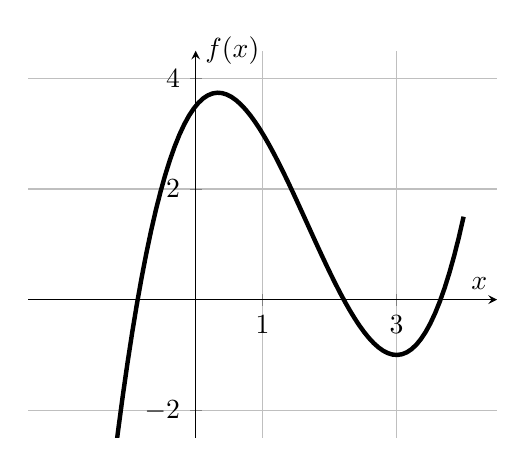
\begin{tikzpicture}[
      declare function={
        func(\x)= 0.5*( \x - 1)^3 - \x^2 + 4;
      }
    ]
      \begin{axis}[height=6.5cm,
        axis lines=center, ymin=-2.5, ymax=4.5, xmin=-2.5, xmax=4.5, xlabel=$x$, ylabel=$f(x)$, ylabel style={right}, ytick={}, xtick={1,3}, grid=major
      ]
        \addplot [domain=-3:4,samples=100, ultra thick]{func(x)};
      \end{axis}

    \end{tikzpicture}

    \columnbreak
    $f'(1)$ is:\\
    because: \\
    \vskip 1em
    $f''(1)$ is: \\
    because: \\
    \vskip 1em
    $f'(3)$ is: \\
    because:  \\
    \vskip 1em
    $f''(3)$ is: \\
    because: \\
    \vskip 1em
  \end{multicols}

\question The function $g$ has a \textbf{derivative} $g'$ with values given in the following table.  Use the table to describe the behavior of $g$, $g'$ and the  $g''$.  That is, can you say whether either of these are positive/negative, increasing/decreasing, or concave up/down?  Briefly explain your answers.

\begin{center}
\begin{tabular}{c|ccccc}
$x$ & 0 & 1 & 2 & 3 & 4 \\ \hline
$g'(x)$ & - 2 & -0.5 & 0.5  & 1  & 1.25
\end{tabular}
\end{center}


\begin{parts}
\part What can you say about $g'(2)$ (which the table says has positive value 0.5)?  Is $g'$ increasing, decreasing, or neither at $x = 2$?
\vfill
\part What can you say about $g''(2)$?  
\vfill
\part What can you say about $g(2)$, the original function whose derivative is given in the table?  (You can determine two of the three characteristics.)
\vfill
\end{parts}

\end{questions}



\newpage

\def\version{B}
%space for name
\noindent {\large\bf Name:} \underline{\hspace{2.5 in}}
\vskip 1em


\begin{questions}
 \question The function $f$ is graphed below.  Use the graph to determine whether the first or second derivatives of $f$ are positive, negative, zero at the given points (circle the correct answer).  Justify your answer by filling in the blanks.

\begin{multicols}{2}
          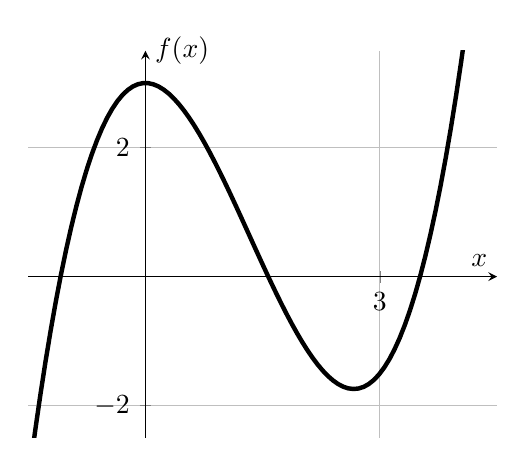
\begin{tikzpicture}[
      declare function={
        func(\x)= 0.5*( \x)^3 - 2*\x^2 + 3;
      }
    ]
      \begin{axis}[height=6.5cm,
        axis lines=center, ymin=-2.5, ymax=3.5, xmin=-1.5, xmax=4.5, xlabel=$x$, ylabel=$f(x)$, ylabel style={right}, ytick={}, xtick={3}, grid=major
      ]
        \addplot [domain=-2:4.5,samples=100, ultra thick]{func(x)};
      \end{axis}

    \end{tikzpicture}

    \columnbreak
    $f'(0)$ is: positive / negative / zero 
    \vskip 1ex
    because near $x=0$, $f(x)$ is \underline{\hspace{1in}} 
    \vskip 1.5ex
    $f''(0)$ is: positive / negative / zero 
    \vskip 1ex
    because near $x=0$, $f(x)$ is \underline{\hspace{1in}} 
    \vskip 1.5ex

    $f'(3)$ is: positive / negative / zero 
    \vskip 1.5ex
    because near $x=3$, $f(x)$ is \underline{\hspace{1in}} 

\vskip 1.5ex

    $f''(3)$ is: positive / negative / zero
    \vskip 1ex
    because near $x=3$, $f(x)$ is \underline{\hspace{1in}} 
  \end{multicols}

\question The function $g$ has a \textbf{derivative} $g'$ with values given in the following table.  Circle the characteristics of $g$, $g'$, and $g''$ that you can conclude from the table at the specified point.

\begin{center}
\begin{tabular}{c|ccccc}
$x$ & 0 & 1 & 2 & 3 & 4 \\ \hline
$g'(x)$ & 3 & 2 & 1.5  & 1  & 0.75
\end{tabular}
\end{center}


\begin{parts}
\part What can you conclude about $g'(2)$?
\vfill
$g'(2)$ is: positive / negative / zero / sign can't be determined.
\vfill
$g'(2)$ is: increasing / decreasing / flat / direction can't be determined.

\vfill
\part What can you say about $g''(2)$?  
\vfill
$g''(2)$ is: positive / negative / zero / sign can't be determined.

\vfill
\part What can you say about $g(2)$, the original function whose derivative is given in the table?
\vfill

$g(2)$ is: positive / negative / zero / sign can't be determined.
\vfill
$g(2)$ is: increasing / decreasing / flat / direction can't be determined.
\vfill
$g(2)$ is: concave up / concave down / linear / shape can't be determined.
\end{parts}

\end{questions}

\newpage

\def\version{C}
%space for name
\noindent {\large\bf Name:} \underline{\hspace{2.5 in}}
\vskip 1em

\begin{questions}

           \question The function $f$ is graphed below.  Use the graph to determine whether the first or second derivatives of $f$ are positive, negative, zero at the given points (circle the correct answer).  Justify your answer by filling in the blanks.

\begin{multicols}{2}
          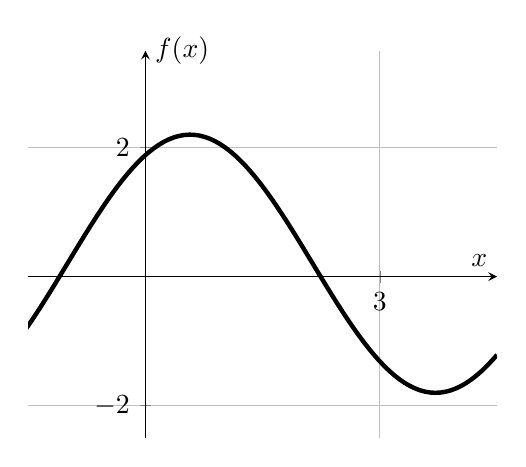
\begin{tikzpicture}[
      declare function={
        func(\x)= 2*sin(deg(\x+1)) + 0.2;
      }
    ]
      \begin{axis}[height=6.5cm,
        axis lines=center, ymin=-2.5, ymax=3.5, xmin=-1.5, xmax=4.5, xlabel=$x$, ylabel=$f(x)$, ylabel style={right}, ytick={}, xtick={3}, grid=major
      ]
        \addplot [domain=-2:4.5,samples=100, ultra thick]{func(x)};
      \end{axis}

    \end{tikzpicture}

    \columnbreak
    $f'(0)$ is: positive / negative / zero 
    \vskip 1ex
    because near $x=0$, $f(x)$ is \underline{\hspace{1in}} 
    \vskip 1.5ex
    $f''(0)$ is: positive / negative / zero 
    \vskip 1ex
    because near $x=0$, $f(x)$ is \underline{\hspace{1in}} 
    \vskip 1.5ex

    $f'(3)$ is: positive / negative / zero 
    \vskip 1.5ex
    because near $x=3$, $f(x)$ is \underline{\hspace{1in}} 

\vskip 1.5ex

    $f''(3)$ is: positive / negative / zero
    \vskip 1ex
    because near $x=3$, $f(x)$ is \underline{\hspace{1in}} 
  \end{multicols}

\question The function $g$ has a \textbf{derivative} $g'$ with values given in the following table.  Circle the characteristics of $g$, $g'$, and $g''$ that you can conclude from the table at the specified point.

\begin{center}
\begin{tabular}{c|ccccc}
$x$ & 0 & 1 & 2 & 3 & 4 \\ \hline
$g'(x)$ & 0.5 & -3 & -2.5  & -1  & 0
\end{tabular}
\end{center}


\begin{parts}
\part What can you conclude about $g'(3)$?
\vfill
$g'(3)$ is: positive / negative / zero / sign can't be determined.
\vfill
$g'(3)$ is: increasing / decreasing / flat / direction can't be determined.

\vfill
\part What can you say about $g''(3)$?  
\vfill
$g''(3)$ is: positive / negative / zero / sign can't be determined.

\vfill
\part What can you say about $g(3)$, the original function whose derivative is given in the table?
\vfill

$g(3)$ is: positive / negative / zero / sign can't be determined.
\vfill
$g(3)$ is: increasing / decreasing / flat / direction can't be determined.
\vfill
$g(3)$ is: concave up / concave down / linear / shape can't be determined.
\end{parts}
\end{questions}


\newpage

\def\version{D}
%space for name
\noindent {\large\bf Name:} \underline{\hspace{2.5 in}}
\vskip 1em


\begin{questions}
  \question The function $f$ is graphed below.  Use the graph to determine whether the first or second derivatives of $f$ are positive, negative, zero at the given points (circle the correct answer).  Justify your answer by filling in the blanks.

\begin{multicols}{2}
          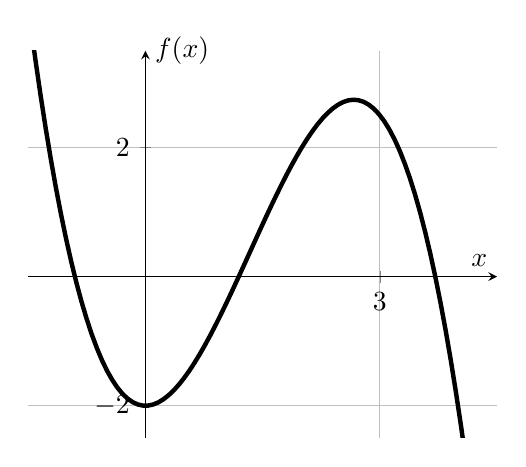
\begin{tikzpicture}[
      declare function={
          func(\x)= -0.5*( \x)^3 + 2*\x^2 - 2;
      }
    ]
      \begin{axis}[height=6.5cm,
        axis lines=center, ymin=-2.5, ymax=3.5, xmin=-1.5, xmax=4.5, xlabel=$x$, ylabel=$f(x)$, ylabel style={right}, ytick={}, xtick={3}, grid=major
      ]
        \addplot [domain=-2:4.5,samples=100, ultra thick]{func(x)};
      \end{axis}

    \end{tikzpicture}

    \columnbreak
    $f'(0)$ is: positive / negative / zero 
    \vskip 1ex
    because near $x=0$, $f(x)$ is \underline{\hspace{1in}} 
    \vskip 1.5ex
    $f''(0)$ is: positive / negative / zero 
    \vskip 1ex
    because near $x=0$, $f(x)$ is \underline{\hspace{1in}} 
    \vskip 1.5ex

    $f'(3)$ is: positive / negative / zero 
    \vskip 1.5ex
    because near $x=3$, $f(x)$ is \underline{\hspace{1in}} 

\vskip 1.5ex

    $f''(3)$ is: positive / negative / zero
    \vskip 1ex
    because near $x=3$, $f(x)$ is \underline{\hspace{1in}} 
  \end{multicols}

\question The function $g$ has a \textbf{derivative} $g'$ with values given in the following table.  Circle the characteristics of $g$, $g'$, and $g''$ that you can conclude from the table at the specified point.

\begin{center}
\begin{tabular}{c|ccccc}
$x$ & 0 & 1 & 2 & 3 & 4 \\ \hline
$g'(x)$ & 1 & 0 & -1  & -2  & -3
\end{tabular}
\end{center}


\begin{parts}
\part What can you conclude about $g'(2)$?
\vfill
$g'(2)$ is: positive / negative / zero / sign can't be determined.
\vfill
$g'(2)$ is: increasing / decreasing / flat / direction can't be determined.

\vfill
\part What can you say about $g''(2)$?  
\vfill
$g''(2)$ is: positive / negative / zero / sign can't be determined.

\vfill
\part What can you say about $g(2)$, the original function whose derivative is given in the table?
\vfill

$g(2)$ is: positive / negative / zero / sign can't be determined.
\vfill
$g(2)$ is: increasing / decreasing / flat / direction can't be determined.
\vfill
$g(2)$ is: concave up / concave down / linear / shape can't be determined.
\end{parts}
\end{questions}

\end{document}
